\documentclass[9pt]{article}
\author{Lawrence Liu}
\usepackage{subcaption}
\usepackage{graphicx}
\usepackage{amsmath}
\usepackage{pdfpages}
\newcommand{\Laplace}{\mathscr{L}}
\setlength{\parskip}{\baselineskip}%
\setlength{\parindent}{0pt}%
\usepackage{xcolor}
\usepackage{listings}
\definecolor{backcolour}{rgb}{0.95,0.95,0.92}
\usepackage{amssymb}
\usepackage{empheq}

\newcommand*\widefbox[1]{\fbox{\hspace{2em}#1\hspace{2em}}}
\lstdefinestyle{mystyle}{
    backgroundcolor=\color{backcolour}}
\lstset{style=mystyle}
\usepackage{wrapfig}
\usepackage{geometry}
\geometry{a4paper,margin=0.075in}
\begin{document}
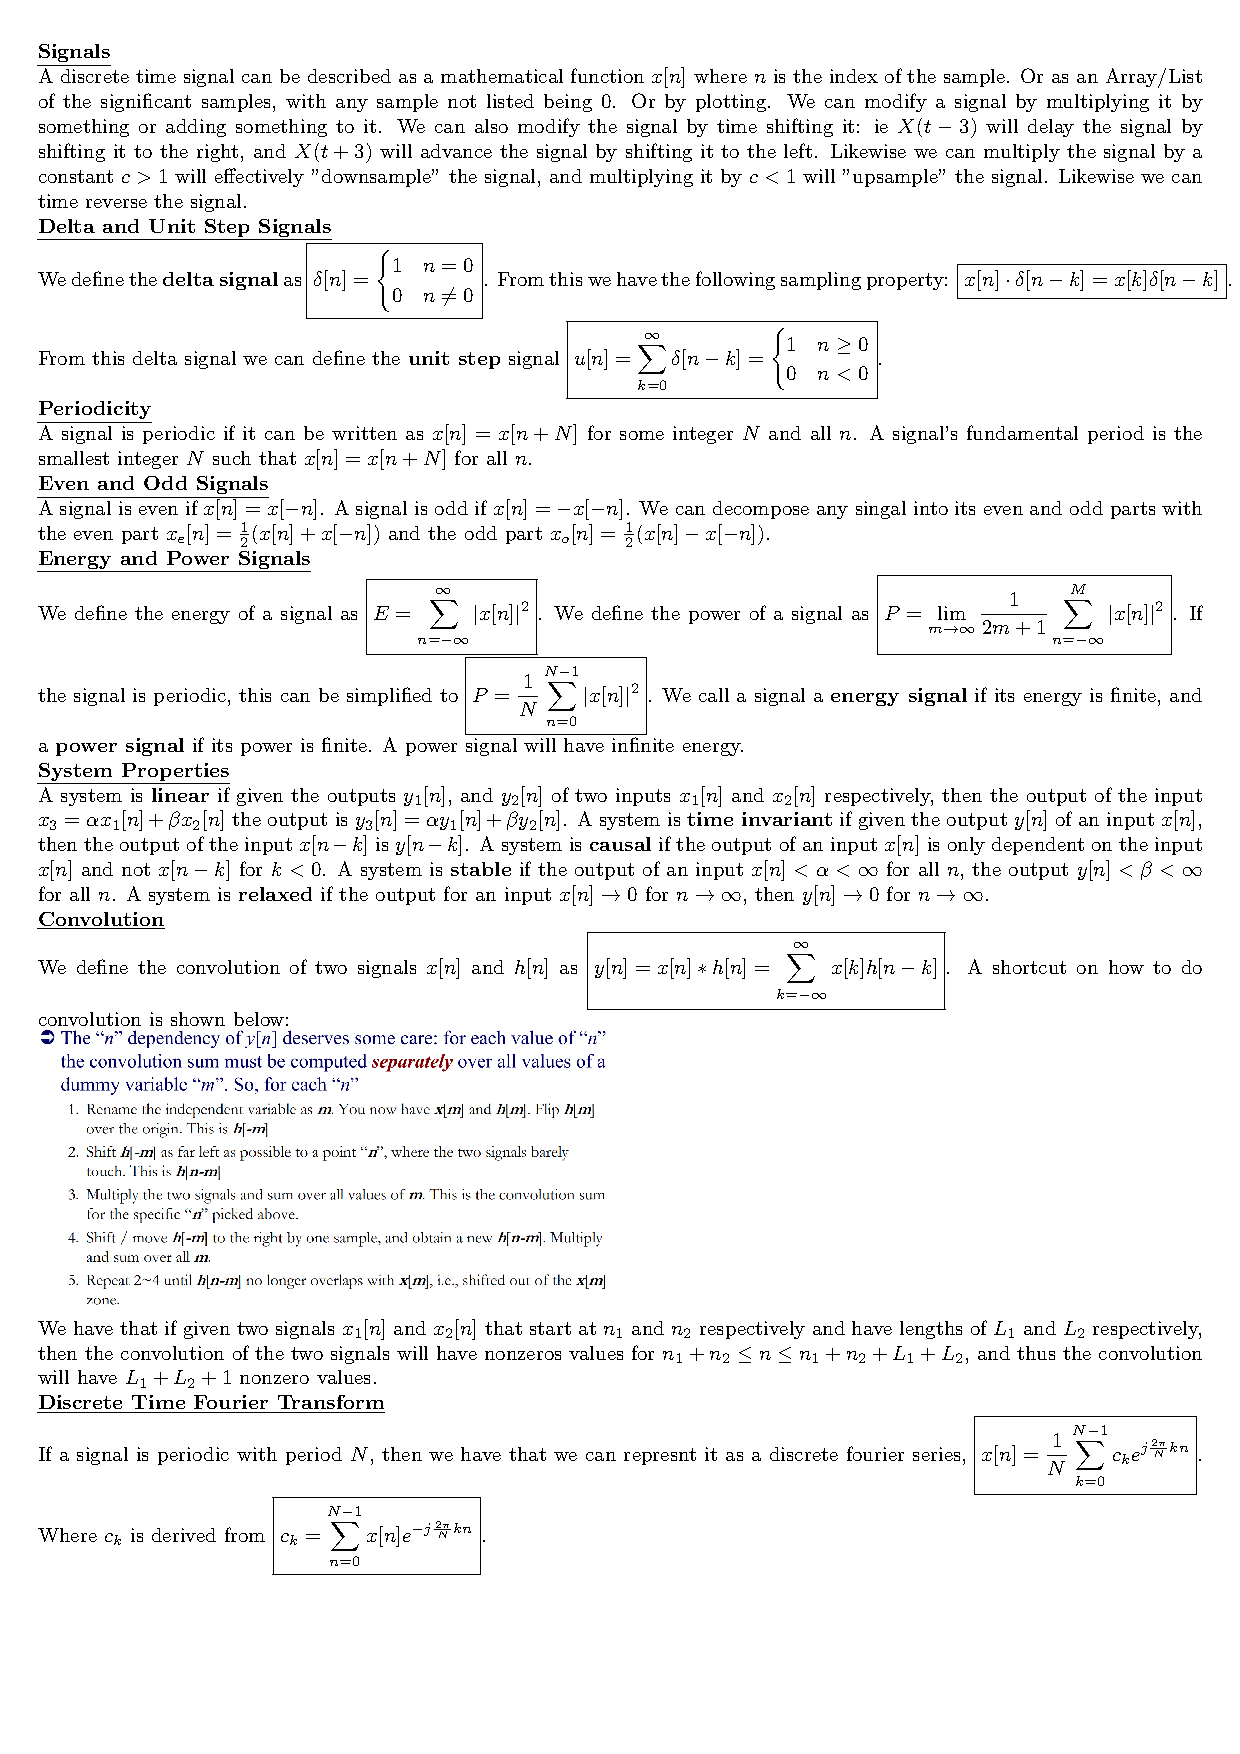
\includepdf[pages=-]{../Midterm/file.pdf}
\underline{\textbf{Periodic Convolution}}\\
Given that two signals $\tilde{x}[n]$ and $\tilde{y}[n]$
 are periodic with period $N$, the we have that the periodic
    convolution of the two signals is given by
    $\boxed{y[n]=\tilde{x}[n]\bigotimes\tilde{y}[n]
    =\sum_{k=0}^{N-1}\tilde{x}[k]\tilde{y}[n-k]}$ it is important 
    to not that 
    $\tilde{x}[n]\bigotimes\tilde{y}[n]=\tilde{x}[n]\bigotimes\tilde{y}[n-N]\neq
    \tilde{x}[n]*\tilde{y}[n]$.\\
\underline{\textbf{Discrete Time Fourier Transform}}\\
We have that the DFTF in general of a signal is: $X_{2\pi}(\omega) =\sum_{n=-\infty}^{\infty}x[n]e^{-j\omega n}$
And its corresponding inverse DTFT is $x[n] = \frac{1}{2\pi}\int_{2\pi}X_{2\pi}(\omega)e^{j\omega n}d\omega$\\
\underline{\textbf{Discrete Fourier Tranform}}\\
Given a signal with a period of $N$, the discrete fourier transform of the signal is 
$X[k]=\sum_{n=0}^{N-1}x[n]e^{-j\frac{2\pi}{N}kn}$ for $0\leq k\leq N-1$. And its inverse is, and with an inverse fourier transform of
$x[n]=\frac{1}{N}\sum_{k=0}^{N-1}X[k]e^{j\frac{2\pi}{N}kn}$. We can 
view the DFT as a sampling of the DTFT with $X[k]=X_{2\pi}(\frac{2\pi}{N}k)$,\\
\underline{\textbf{Linear Algebra for the DFT}}\\
We can express the DFT as a matrix multiplication, where
the vector $X_k$ is the DFT of the signal represented by the vector $x_n$
of size n then we have that letting $W=\begin{bmatrix}
    1 & 1 & 1 & \cdots & 1 \\
    1 & \omega^{1} & \omega^{2} & \cdots & \omega^{N-1} \\
    \vdots & \vdots & \vdots & \ddots & \vdots \\
    1 & \omega^{N-1} & \omega^{2(N-1)} & \cdots & \omega^{(N-1)^2}
\end{bmatrix}$ we get that
$\boxed{X_k=Wx_n}$, where $\omega=e^{-j\frac{2\pi}{N}}$. An important thing to note about $W$ is that it 
is symetric, therefore the inverse fourier transform is just 
$\boxed{x_n=\frac{1}{N}W^H X_k}$
where $W^H$ is the conjugate transpose of $W$, or since 
$W$ is symetric, $W^H=W^*$, where $W^*$ is the conjugate of $W$.\\
\underline{\textbf{FFT}}\\
The naive implementation of the DFT is $O(N^2)$, however we can use the
property that we can rewrite the DFT as 
$X_k=\sum_{m=0}^{N/2-1}x_{2m}e^{-j\frac{2\pi}{N}k2m}+\sum_{m=0}^{N/2-1}x_{2m+1}e^{-j\frac{2\pi}{N}(2m+1)k}
=\sum_{m=0}^{N/2-1}x_{2m}e^{-j\frac{2\pi}{N}k2m}+e^{-j\frac{2\pi}{N}k}\sum_{m=0}^{N/2-1}x_{2m+1}e^{-j\frac{2\pi}{N}(2m)k}$
Therefore we can break the DFT into two smaller DFTs, and then combine them to get the DFT of the original signal.
repeating this we get that we can optimize the FFT's complexity to 
$O(NlogN)$, where $N$ is the length of the signal.\\
\underline{\textbf{Z transform}}\\
The z transform of a signal is given by $X(z)=\sum_{n=-\infty}^{\infty}x[n]z^{-n}$. We define the 
reigon of convergence as the set of $z$ such that this sum exists. 


\end{document}

